\documentclass[verslag.tex]{subfiles} 
\begin{document}

\part{Interface module}
\label{interface}

\chapter{Hardware}

Zoals uit de doeken gedaan in deel \ref{ontwerp}, zullen we voor de interface gebruik maken van een AVR microcontroller met daarop de V-USB firmware om low speed datacommunicatie te verwezenlijken met minimale periferie.

\section{Microcontroller}

Door het gebruik van de V-USB bibliotheek moeten we ons beperken tot AVR microcontrollers, maar binnen die familie is het aanbod nog altijd zeer groot. Om een goede selectie te maken, moeten we logischerwijs rekening houden met de eisen die de V-USB bibliotheek stelt:
\begin{itemize}
\item Flash: tenminste 2 kB;
\item RAM: tenminste 128 bytes;
\item Kloksnelheid: 12.8 of 16.5 MHz bij gebruik van een interne oscillator, en ook 12, 15, 16 of 20 MHz indien we gebruik maken van een extern kristal\footnote{Dit omdat enkel de 12.8 en 16.5 MHz frequenties een deviatie van 1\% toelaten, en het bij een interen oscillator onmogelijk is om een heel precieze afstelling te bekomen.};
\item Poorten: exact 2, beide met een interruptlijn.
\end{itemize}

We willen echter ook een uitbreidbare module realiseren. Momenteel hebben we slechts 4 knoppen aan te sluiten, maar mogelijks worden dit er later meer. Daarom zullen we de ruimte laten voor drie extra knoppen, wat we eenvoudig kunnen realiseren met slechts 4 poorten door het signaal te multiplexen. Als we tenslotte overlappingen negeren, volstaat het zelfs om maar 3 poorten te gebruiken.

Tenslotte zou het ook interessant zijn moest de microcontroller voorzien van \ac{isp} headers, waardoor de firmware van de module achteraf nog kan vernieuwd worden zonder daarvoor de microcontroller te moeten verwijderen uit de module. Indien we het echter mogelijk willen maken om de chip te herprogrammeren via \ac{isp}, kunnen we geen gebruik maken van \ac{hvsp} (waarvoor de chip fysiek moet geplaatst in een \ac{hvsp} programmer moet geplaatst worden). \ac{hvsp} is een speciale methode om een microcontroller te programmeren, waarbij het mogelijk is om voordien ingestelde \emph{fuses} opnieuw in te stellen. Zo is er bijvoorbeeld de fuse die de \code{RESET}-poort (aanwezig op elke AVR microcontroller) configureert als een reguliere input/output poort. Deze fuse kan initieel wel ingesteld worden via \ac{isp}, maar heeft als consequentie dat de chip nadien niet meer kan geherprogrammeerd worden, tenzij door gebruik te maken van \ac{hvsp} waarmee de fuse in kwestie opnieuw ingesteld kan worden. Hierdoor is het dus onmogelijk om de \code{RESET}-poort te gebruiken als reguliere poort.

Een microcontroller die voldoet aan deze eisen, is de \strong{AtTiny45}. Deze heeft de volgende relevante specificaties:
\begin{itemize}
\item Flash: 4 kB;
\item RAM: 256 bytes;
\item EEPROM: 256 bytes;
\item ISP: aanwezig;
\item Kloksnelheid: 10 MHz voor de low-voltage versie, en tot 20 MHz voor de reguliere versie;
\item Interne oscillator: gekalibreerd voor 8 MHz;
\item Voedingsspanning: 1.8-5.5 volt voor de low-voltage versie, en 2.7-5.5 volt voor de reguliere versie.
\end{itemize}

\subsection{Kloksnelheid}

Om het aantal componenten te minimaliseren, zouden we de module graag realiseren zonder gebruik te maken van een externe oscillator. De interne oscillator is echter enkel gekalibreerd om op 8 MHz te werken, wat niet bruikbaar is in combinatie met V-USB. Om toch een bruikbare frequentie te bekomen, maken we gebruik van een kalibratiemechanisme terug te vinden in het \makeurl{http://www.obdev.at/products/vusb/easylogger.html}{EasyLogger} voorbeeldproject.

De eerste stap bestaat uit het kalibreren van de interne oscillator tot een frequentie van 8.25 MHz, dit door te vergelijken met binnenkomende \ac{usb} frames en binair te zoeken naar een optimale waarde voor het \code{OSCCAL} oscillator kalibratieregister. Hierdoor zal de \ac{pll} clock, steeds gelijk aan een achtvoudige versnelling van de interne oscillator, ingesteld worden op 66 MHz. Indien we tenslotte de \code{CLKSEL} fuse bij het programmeren instellen op $0001$ zal de systeemklok gelijk ingesteld worden aan de \ac{pll} clock gedeeld door 4, wat overeen komt met 16.5 MHz, een frequentie die we kunnen gebruiken in combinatie met de V-USB code.

\subsection{Voeding}

Aangezien de kloksnelheid waarop onze microcontroller zal draaien, 16.5 MHz, groter is dan 10 MHz, zullen we geen gebruik kunnen maken van de low-voltage versie. Meer nog: om een kloksnelheid groter dan 10 MHz te bekomen, zal de voedingsspanning zelfs tussen de 4.5 en 5.5 volt moeten bedragen. Op het eerste zicht vormt dit geen probleem, we kunnen immers de \ac{usb} voedingslijn (mits ontkoppeling) direct gebruiken om de microcontroller te voeden. Maar zoals uit de volgende paragraaf zal blijken, zou het zo ook zijn voordelen kennen moesten we de microcontroller kunnen voeden met een lagere spanning.

Natuurlijk zullen we ook de voedingsspanning ontkoppelen, en dit op twee vlakken. Om de hoogfrequente schakelpieken van de digitale microcontroller af te vlakken, plaatsen we een 100 nanofarad condensator tussen de voedingslijn en de grondplaat. Het valt op te merken dat we die condensator zo dicht mogelijk tegen de voedingspin van de microcontroller willen plaatsen, dit om parasitaire capaciteiten te vermijden. Vervolgens willen we ook eventuele ongerelmatigheden afvlakken (hetzij van de spanningsbron uit, hetzij veroorzaakt door een plotse toename in verbruik), waarvoor we een 10 microfarad condensator plaatsen aan de kant van de \ac{usb} connector. De waarde van 10 microfarad is niet uit de lucht gegrepen: ze is relatief hoog om de typisch laagfrequentere pieken die een spanningsbron genereert af te vlakken, en tegelijk is het ook het maximum dat de \ac{usb} specificatie \makeurl{http://www.beyondlogic.org/usbnutshell/usb2.shtml}{toelaat}.

\begin{figure}
	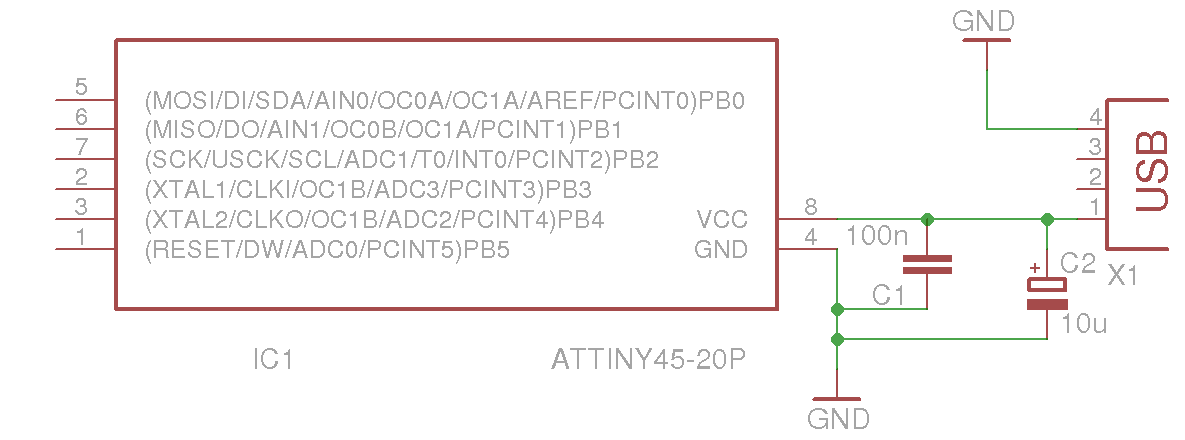
\includegraphics[width=\textwidth]{afbeeldingen/circuit_voeding}
	\caption{Voedingscircuit}
\end{figure}

\subsection{Signalen}

\ac{usb} datacommunicatie verloopt steeds over een \emph{twisted-pair}, op een differentiële manier. Dit betekent dat een signaalbit afgeleid wordt uit het potentiaalverschil tussen de twee signaaldragers, en dat die binnen een \ac{usb}-kabel steeds getwist zijn. Het voordeel van het twisten is dat eventuele ruis grotendeels evenredig verdeeld is over beide kabels, waardoor het potentiaalverschil tussen beide vaak onveranderd blijft. Hierdoor is differentiële dataoverdracht over een twisted-pair veel beter bestand tegen elektromagnetische ruis.

Eerst en vooral zorgen we voor een stroombeperking op de signaaldragers. Hiertoe zullen we tussen de signaalpin en de \ac{usb} connector een weerstand van 68 ohm plaatsen, die ervoor zorgen dat er nooit meer dan 50 milliampères zal vloeien.

De specifieke elektrische kenmerken van de implementatie in het \ac{usb} protocol zijn echter vervelend voor gebruik in combinatie met de meeste digitale componenten. Zo wordt een hoog signaal gekenmerkt door een differentieel signaal van 2.8 tot 3.6 volt, terwijl voor een laag signaal 0 tot 0.3 volt te detecteren valt. Voor toekomende signalen (het twisted-pair is immers half-duplex) vormen deze waarden geen probleem: de meeste microcontrollers, waaronder de gebruikte AtTiny45, herkennen een signaal van 3.3 volt als een hoog signaal (hoewel de specificatie slechts een bereik vastlegt, sturen de meeste hosts exact 3.3 volt) . Wat wel een probleem vormt, zijn de uitgaande signalen. Aangezien onze microcontroller gevoed wordt door 5 volt, kennen de signalen tevens een spanning van 5 volt, wat ruimschoots buiten het opgelegde bereik valt.

Een mogelijke oplossing bestaat eruit de \strong{voedingsspanning van de microcontroller te verlagen} tot 3.6 volt. Aangezien de spanning die de microcontroller gebruikt op de signaalpinnen min of meer gelijk is aan de voedingsspanning, en de AtTiny45 genoeg heeft aan slechts 1.8 tot 2.7 volt (afhankelijk van de uitvoering), zou dit het probleem direct oplossen. Er zou enkel nood zijn aan een spanningsregulator om de voedingsspanning te reduceren tot 3.6 volt, wat dan wel een \emph{low-drop} regulator zou moeten zijn (omdat gewone regulators meestal een initiële drop van 2 volt kennen). Een minder robuust vervangt deze regulator door twee diodes, waardoor een voltage drop van 1.2 tot 1.4 volt bekomen wordt.
Jammer genoeg kunnen we geen van deze oplossingen gebruiken, omdat de microcontroller op 16.5 MHz zal draaien waarvoor we een voedingsspanning tussen de 4.5 en 5 volt nodig hebben.

Een alternatief bestaat eruit om het \textbf{spanningsniveau van de signaalpinnen te reguleren}. Hiertoe raadt de \makeurl{http://vusb.wikidot.com/hardware}{V-USB wiki} bijvoorbeeld aan om gebruik te maken van 3.6 volt zenerdioden. Zenerdioden hebben immers de eigenschap dat ze, van zodra de zenerspanning bereikt is, in sper geleidt alsook dat de spanning erover relatief constant blijft. Meer concreet houdt dit in dat, indien we de signaalpinnen via een zenerdiode in sper verbinden met de grondplaat, de spanning van het signaal gereduceerd wordt tot 3.6 volt. Deze opzet kent echter ook enkele problemen. Zo kan het moeilijk zijn om de exacte combinatie van parameters vast te leggen, zenerdiodes komen immers in soorten en maten. Een ander nadeel zijn de hoge stromen veroorzaakt door de zenerdiode. Wanneer de diode immers een hoog 5 volt signaal reduceert tot 3.6 volt, zal de overige 1.4 volt over de 68 ohm weerstanden tussen de microcontroller en de \ac{usb} host komen te staan, wat zorgt voor liefst 20 milliampères over de signaaldrager.

Tenslotte moeten we nog voorzien in een \emph{setting weerstand} die een spanning plaatst op de negatieve signaaldrager. Deze pull-up weerstand maakt aan de \ac{usb} host duidelijk te maken dat er een \ac{usb} 1.1 toestel aangesloten is (weliswaar actief in \emph{low speed} modus). Voor een 5 volt lijn kan dit gerealiseerd worden met een 1k8 of 2k2 ohm weerstand.

\begin{figure}
	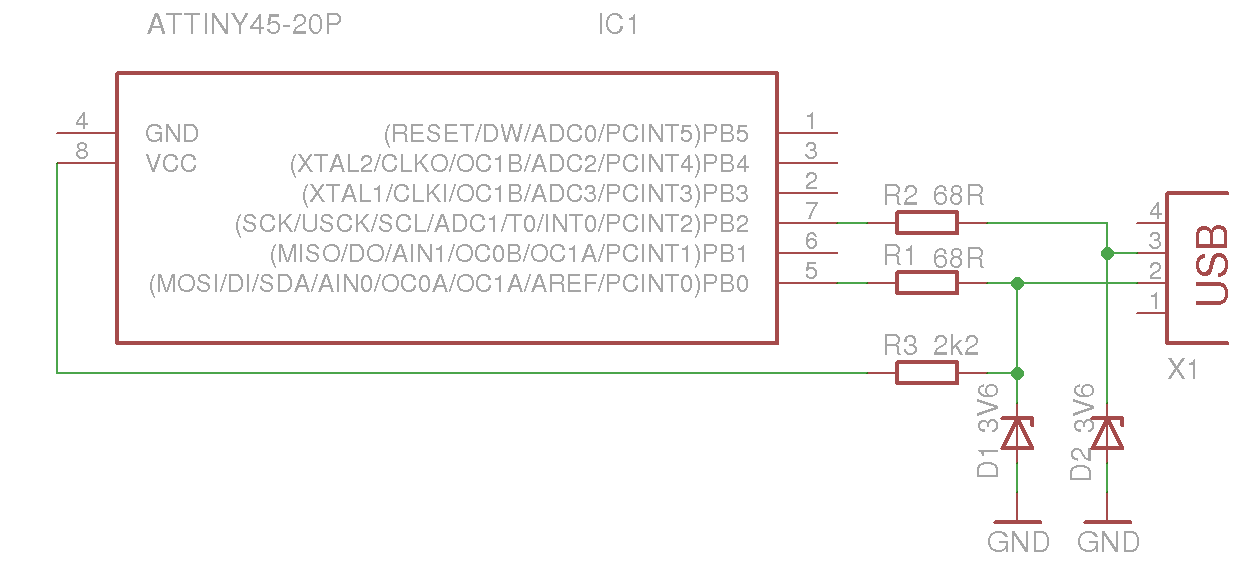
\includegraphics[width=\textwidth]{afbeeldingen/circuit_signaal}
	\caption{Signaalconversie}
\end{figure}

\subsection{\acs{isp}}

Het invoegen van een \ac{isp} header is niet veel werk: we dienen gewoon te voorzien in een connector, en de pinnen ervan correct doorverbinden met de juiste pinnen van de microcontroller.

TODO: programmeren als systeem actief is?

\begin{figure}
	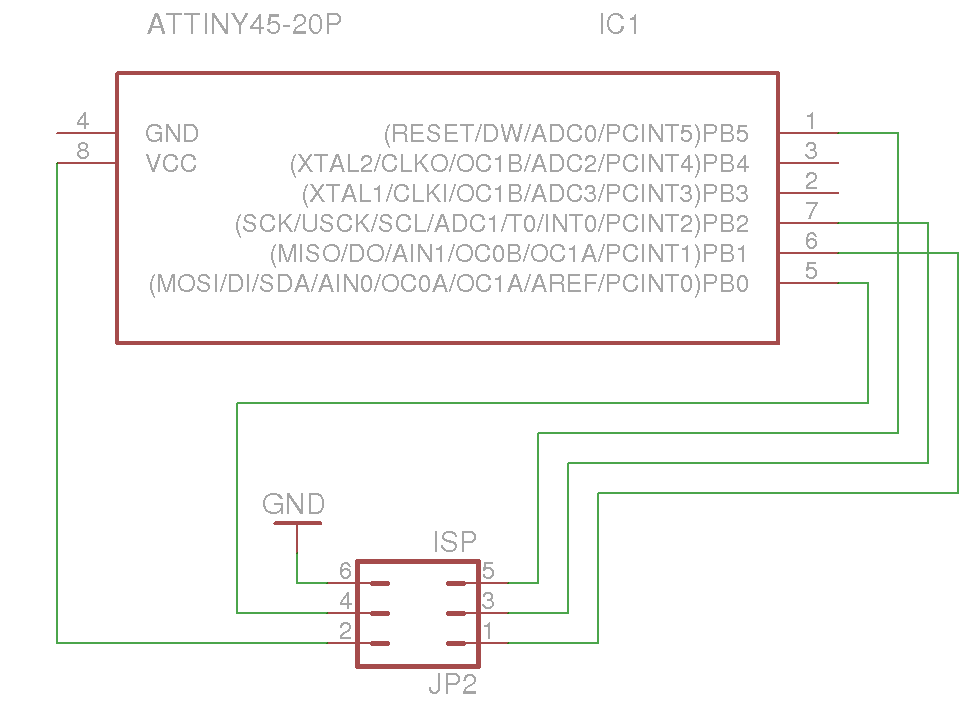
\includegraphics[width=\textwidth]{afbeeldingen/circuit_isp}
	\caption{\acs{isp} connector}
\end{figure}

\section{Schakelaars}

De schakelaars bevinden zich fysiek niet op de interface module, maar zijn reeds ingebouwd in de bestaande kasten. Daarom zullen we een systeem moeten bedenken om de bestaande schakelaars op een handige manier op de module aan te sluiten. Tevens moeten we de knoppen zodanig verbinden dat er uitbreidingsmogelijkheden zijn.

Om de bestaande schakelaars op een eenvoudige manier aan te sluiten, zullen we de interface module voorzien van een connector waarop we eenvoudig knoppen kunnen op aansluiten. De meest robuuste oplossing hierbij is een connector die vastklikt op de module, waardoor die niet per toeval kan loskomen. Dergelijke connectors zijn echter vrij specifiek, en vereisen per aan te sluiten schakelaar een element op de printplaat. Een alternatief, dat als voordeel heeft dat het geen speciale connector aan de kant van de knoppen vereist, zijn vijs-connectors. Hierbij worden de losse draden van de knoppen via een vijsaansluiting op de printplaat bevestigd. Hoewel dit al een betere oplossing is, vereist het nog altijd een connector op de printplaat voor elke knop, en neemt het vast- en losvijzen van de kabels ook meer tijd in beslag dan het aansluiten van een eenvoudige connector. Daarom hebben we gekozen voor de alombekende \emph{jumpers}. Deze makkelijk te vinden connectors kunnen eenvoudig aan het kabelpaar van de knoppen bevestigd worden door middel van een krimptang. Aan de kant van de printplaat is het ook een eenvoudigere oplossing, daar het mogelijk is de aansluitingen voor alle schakelaars door middel van een enkel blok jumpers te realiseren. Het enige nadeel is dat een aangesloten connectors niet zo vast zitten: bij gebrek aan weerhaak of ander systeem kan de kabel relatief gemakkelijk loskomen.

Om de aansluitingen op de printplaat eenvoudig te houden, zullen we werken met een \emph{active-low} mechanisme: een knop zal wanneer ingedrukt bepaalde signaallijnen doorverbinden met de elektrische grond. Om er voor te zorgen dat er een hoog signaal gemeten wordt wanneer er geen verbinding is met de elektrische grond, maken we gebruik van de interne pull-up die beschikbaar is voor elke poortpin: dit is een weerstand tussen de $20$ en $50$ kilo-ohm die de poortpin intern doorverbindt met de positieve voedingslijn. Hierdoor zal bij afwezigheid van een externe verbinding de spanning op de poortpin gelijk zijn aan de voedingsspanning, wat gedetecteerd wordt als een hoog signaal. Wanneer we echter de poortpin zullen doorverbinden naar de elektrische grond, zal deze pull-up weerstand zorgen voor een stroom tussen de $0.1$ en $0.25$ milliampères.

Er is echter een bijkomend probleem: we hebben maar 3 poortpinnen tot onze beschikking, waardoor het niet mogelijk is elke knop door te verbinden met een eigen poortpin. De eenvoudige oplossing hierbij is het gebruik van een multiplexer: 2 select-lijnen en 1 datalijn maakt het mogelijk om 4 schakelaars uit te lezen. We willen echter meer knoppen kunnen aansluiten, zonder daarbij extra poortpinnen nodig te hebben. Daarom zullen we zelf het signaal multiplexen, waarbij we meer schakelaars kunnen toelaten door geen gebruik te maken van een selectiemechanisme, maar de signalen direct door te linken naar de poortpinnen. Het nadeel aan deze opzet is dat de signalen kunnen overlappen, zo zullen we bij het indrukken van meerdere knoppen tegelijkertijd niet kunnen uitmaken welke knoppen juist ingedrukt zijn.

De realisatie van een dergelijke multiplexer lijkt eenvoudig, maar er is een belangrijk detail dat we moeten opmerken. Aangezien de verschillende poortpinnen verbonden zijn met verschillende knoppen, kan er bij het indrukken van een enkele schakelaar stroom terugvloeien via de contactpunten van diens signaallijnen met andere knoppen van een totaal ongerelateerde poortpin, zoals te zien is op figuur \ref{fig:circuit_schakelaars_foutief}. Om dit te vermijden moeten we overal waar er twee signaallijnen met elkaar verbonden zijn, een diode plaatsen zodat er geen stroom kan terugvloeien naar een vorig verbindingspunt. Hiervoor hebben we een reguliere diode nodig, waarbij geen speciale eisen gesteld worden. Daarom kiezen we voor de 1N4148, een populaire diode die vaak gebruikt wordt voor het schakelen van digitale signalen. Zoals we kunnen opzoeken in het stroom-spanningsdiagram van deze diode, zorgt ze bij een stroom tussen $0.1$ en $0.25$ milliampères (gegenereerd door de pull-up weerstand binnen de microcontroller) voor een spanningsval van $0.5$ volt.

\begin{figure}
	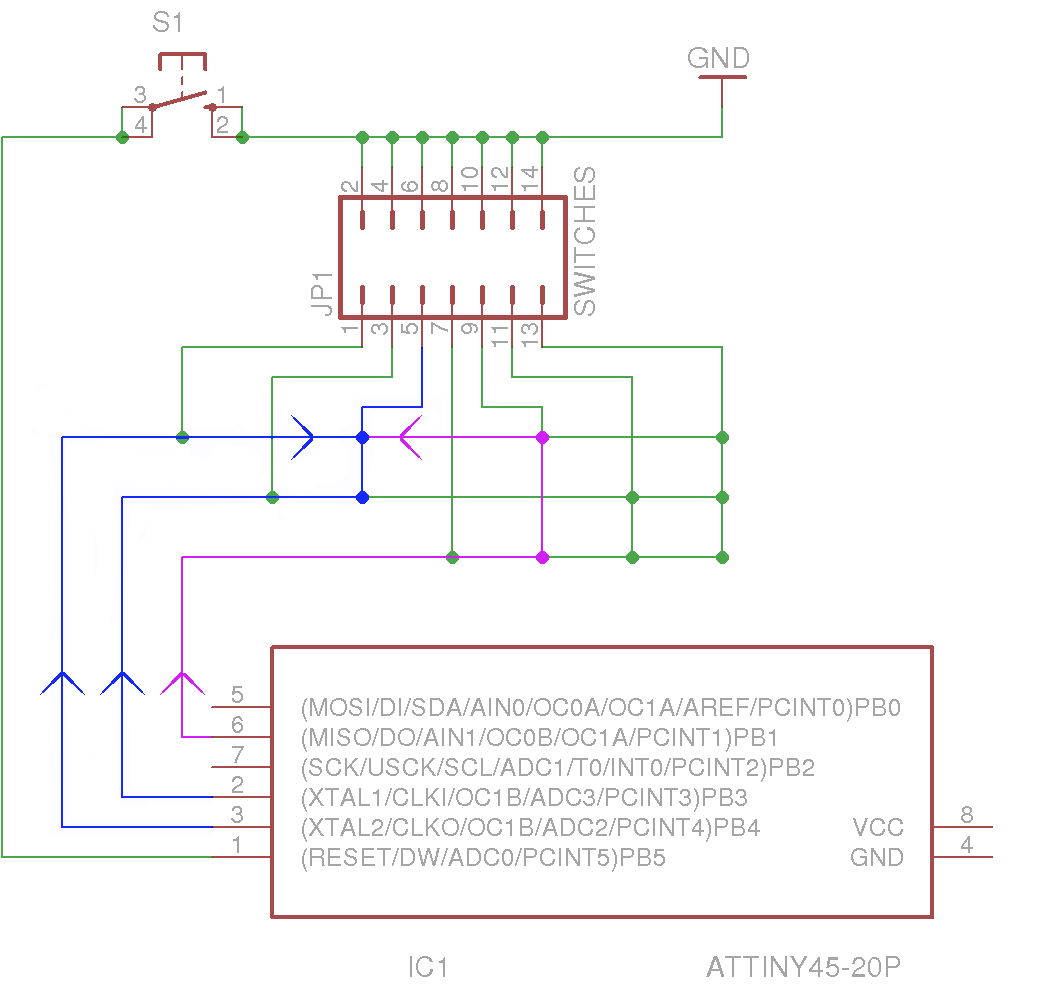
\includegraphics[width=\textwidth]{afbeeldingen/circuit_schakelaars_foutief}
	\caption{Circuit en connector voor schakelaars zonder dioden, en aanduiding van voorbeeldstromen daarbij}
	\label{fig:circuit_schakelaars_foutief}
\end{figure}

We kunnen wel niet zomaar dioden op de signaallijnen plaatsen. Als we dit wel zouden doen, zou de het volledige spanningsverschil tussen de elektrische grond en de poortpin (wat $5$ volt bedraagt, dankzij de interne pull-up) over de diode geplaatst worden, waardoor die beschadigd zou worden. Dit zou opgelost kunnen worden door bij elk van de drie poortpinnen een extra beschermingsweerstand te plaatsen, waardoor de overmatige spanning over deze weerstand zou komen te staan en de dioden slechts het spanningsverschil waarvoor ze gemaakt zijn zouden moeten verwerken. Het berekenen van de waarde van deze weerstand zou wel enig werk vereisen, daar we moeten zorgen dat de spanning die aan het hoogimpedant meetcircuit aangelegd wordt zich binnen het bereik van een laag signaal bevindt. De datasheet van de microcontroller stelt zo dat een laag signaal gedetecteerd wordt tussen $0$ volt en $0.6$ keer de bronspanning. Aangezien de microcontroller zich rechtstreeks voedt met de USB bronspanning, dewelke $5$ volt bedraagt, moet de spanning aan het meetcircuit vallen tussen $0$ en $3$ volt.

Als we echter nauwkeuriger kijken naar de werking van de interne pull-up (figuur \ref{fig:avr_pullup}), zien we dat deze reeds op zichzelf functioneert als een beschermingsweerstand. In het slechtste geval bijvoorbeeld, waarbij er zich na de pull-up nog drie dioden met elk een spanningsval van $0.5$ volt bevinden, zal er zich zo slechts $1.5$ volt op de signaallijn bevinden, wat ruim binnen de grenzen voor detectie van een laag signaal bevindt. Aangezien de weerstand tevens voldoende groot is, moeten we niet zorgen voor een extra stroomreductie en verdwijnt elk nut van een extra beschermingsweerstand.

\begin{figure}
	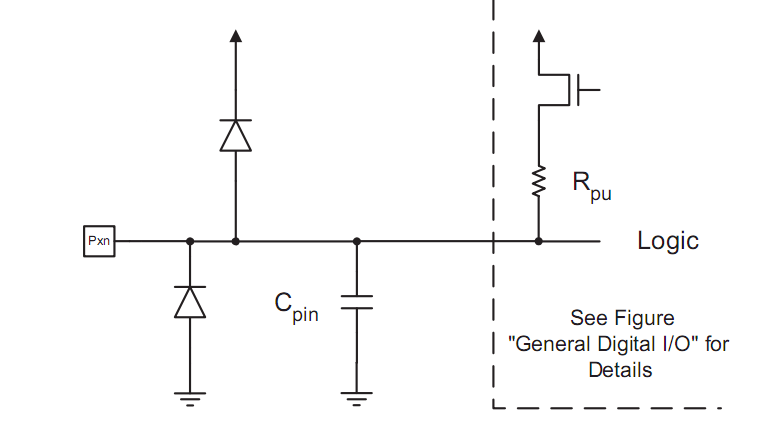
\includegraphics[width=\textwidth]{afbeeldingen/avr_pullup}
	\caption{Pull-up weerstand binnenin een AVR microcontroller}
	\label{fig:avr_pullup}
\end{figure}

\begin{figure}
	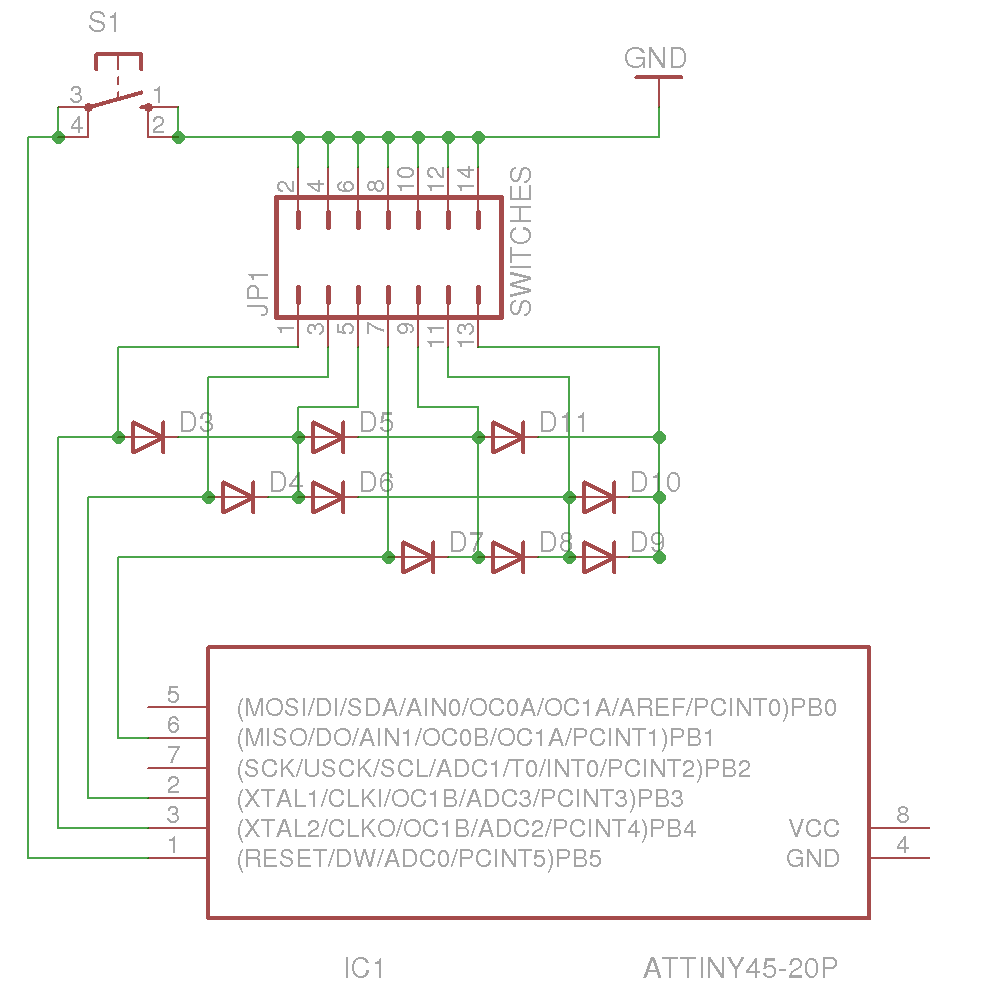
\includegraphics[width=\textwidth]{afbeeldingen/circuit_schakelaars}
	\caption{Circuit en connector voor schakelaars}
\end{figure}

\section{Productie}

\begin{figure}
	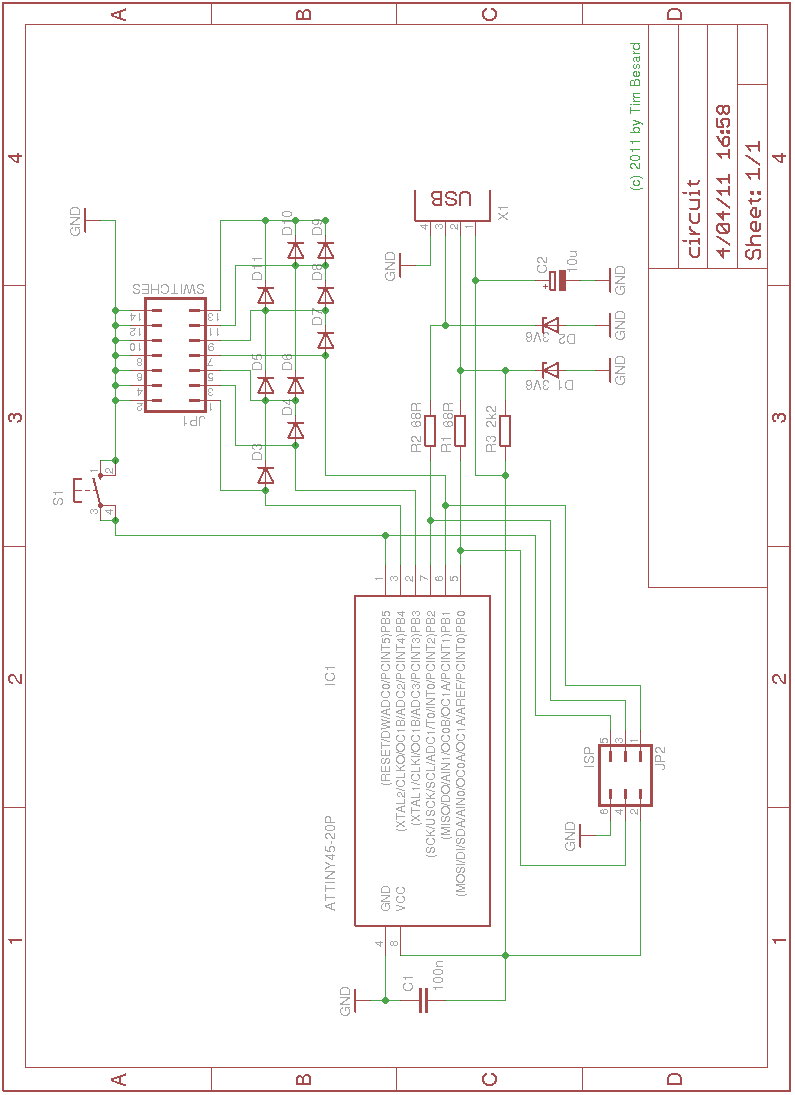
\includegraphics[width=\textwidth]{afbeeldingen/circuit}
	\caption{Uiteindelijk circuit}
\end{figure}

\chapter{Firmware}

\end{document}

